\documentclass[t,handout]{beamer}

\usepackage[utf8]{inputenc}
\usepackage{ngerman}
\usepackage[T1]{fontenc}
\usepackage{graphicx}
\usepackage{ifthen}
\usepackage{listings}
\usepackage{array}
%\usepackage{tikz}
%\usetikzlibrary{calc}
%\usetikzlibrary{shapes.symbols}


\input{beamerHtwFolien}
%\input{../macros}
%\input{tikzBase}

\title{JavaScript-basierte Entwicklung und SAP HANA}
\subtitle{Ausgewählte Datenbankkonzepte/-techniken}
\author[Ingo Claßen]{Prof.~Dr.~Ingo Claßen}
\institute[HTW Berlin]{Hochschule für Technik und Wirtschaft Berlin}
\date{}
%\titlegraphic{\small Kurzpräsentation}

\begin{document}

%\begin{frame}[plain]
%  \titlepage
%\end{frame}

\begin{frame}[plain]
  \maketitle
  \vspace*{-1cm}
  \tableofcontents
\end{frame}

\section{Asynchrone Funktionen}
\begin{frame}{Asynchrone Funktionen}
  \begin{itemize}
    \item Aufruf von Funktionen ohne Blockierung des Aufrufers
    \item Kein Warten auf die Antwort der aufgerufenen Funktion
    \item Zeitliche Versetzung der Ergebnisbereitstellung
    \item Typische Beispiele: File IO, DB-Aufrufe, Aufruf Web Services
    \item f1: Platzhalter für diese Arten von Funktionen\\[.2cm]
          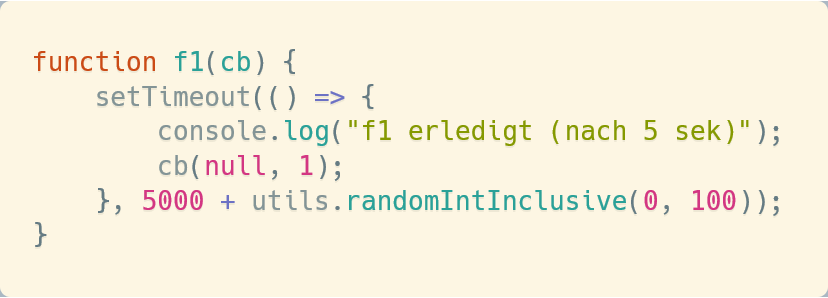
\includegraphics[scale=.28]{fig/async1.png}
    \item Callback-Funktion cb: (err, result) => body
  \end{itemize}
\end{frame}

\begin{frame}{Asynchrone Ausführungsreihenfolge}
  \begin{center}
    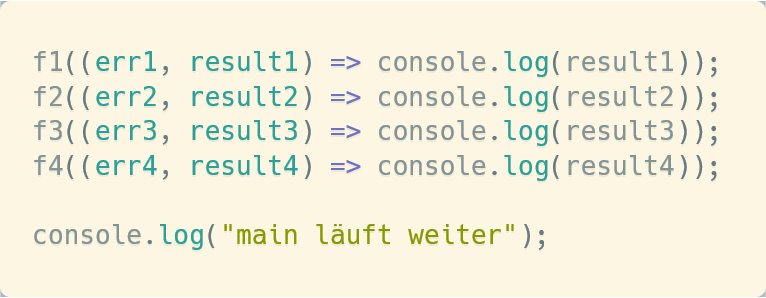
\includegraphics[scale=.28]{fig/async2.png}\\[.2cm]
    \begin{columns}
      \begin{column}{0.48\textwidth}
        Erster Durchlauf\\[.2cm]
        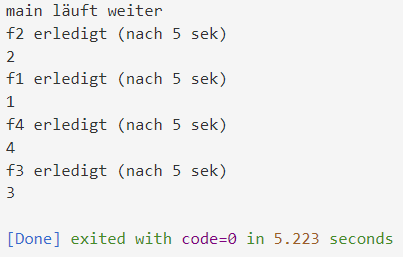
\includegraphics[scale=.5]{fig/async3.png}
      \end{column}
      \begin{column}{0.48\textwidth}
        Erneuter Durchlauf\\[.2cm]
        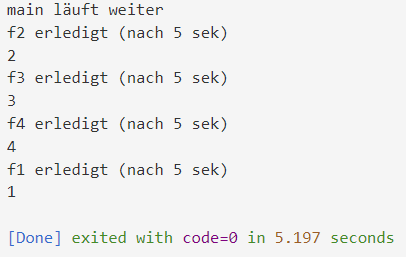
\includegraphics[scale=.5]{fig/async4.png}
      \end{column}
    \end{columns}
  \end{center}
\end{frame}

\begin{frame}{Node.JS-System}
  \begin{center}
    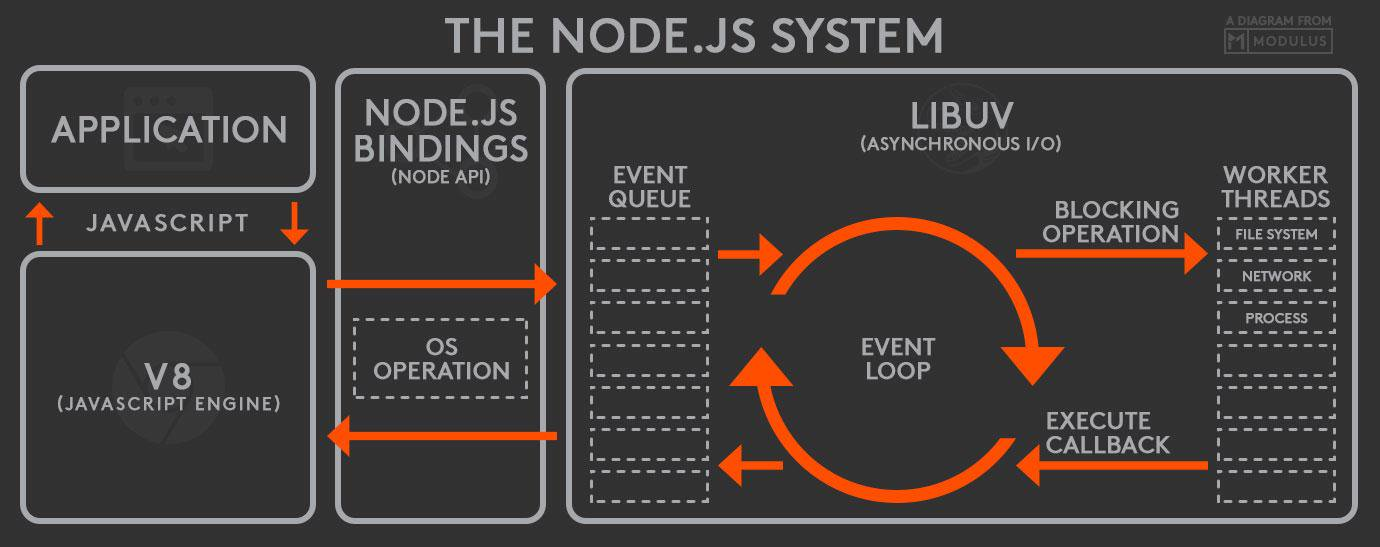
\includegraphics[scale=.25]{fig/nodejs-system1.jpg}
  \end{center}
\end{frame}

\begin{frame}{Synchrone Ausführungsreihenfolge -- Callback Hell}
  \begin{center}
    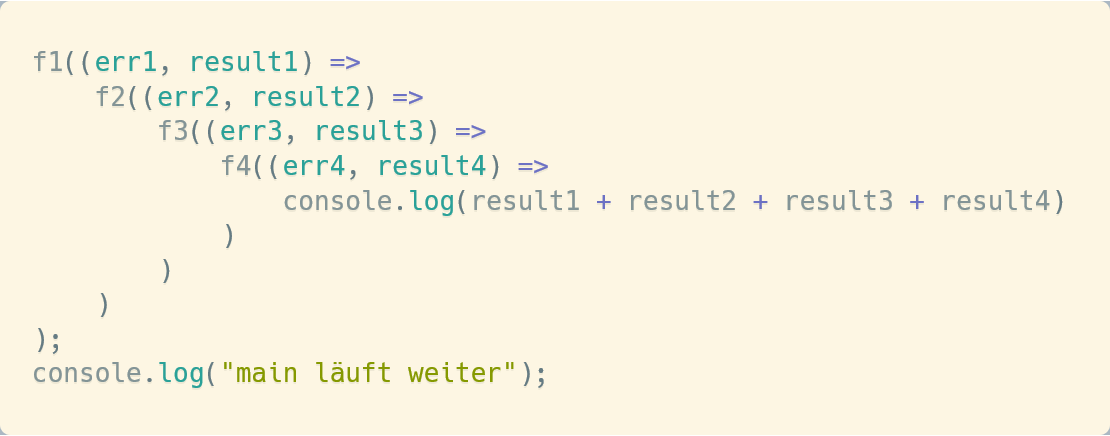
\includegraphics[scale=.28]{fig/async5.png}\\[.1cm]
    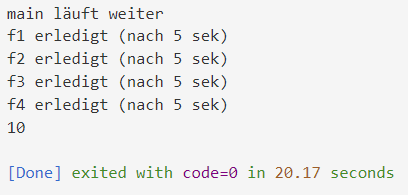
\includegraphics[scale=.6]{fig/async6.png}
  \end{center}
\end{frame}

\section{Promises}
\begin{frame}{Promises}
  \begin{center}
    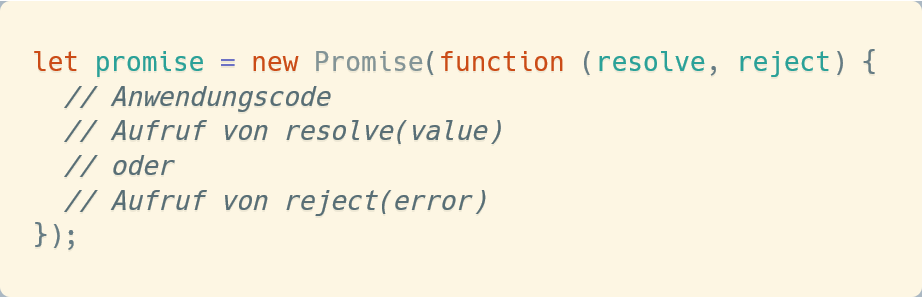
\includegraphics[scale=.28]{fig/promises1.png}\\[.2cm]
    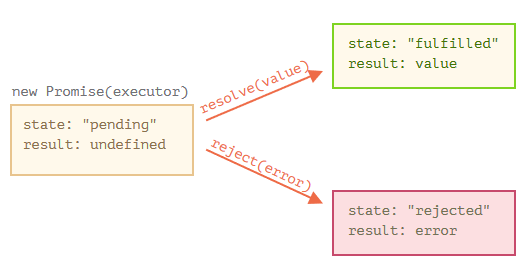
\includegraphics[scale=.6]{fig/promises2.png}
  \end{center}
\end{frame}

\begin{frame}{Promises Ausführung}
  \begin{center}
    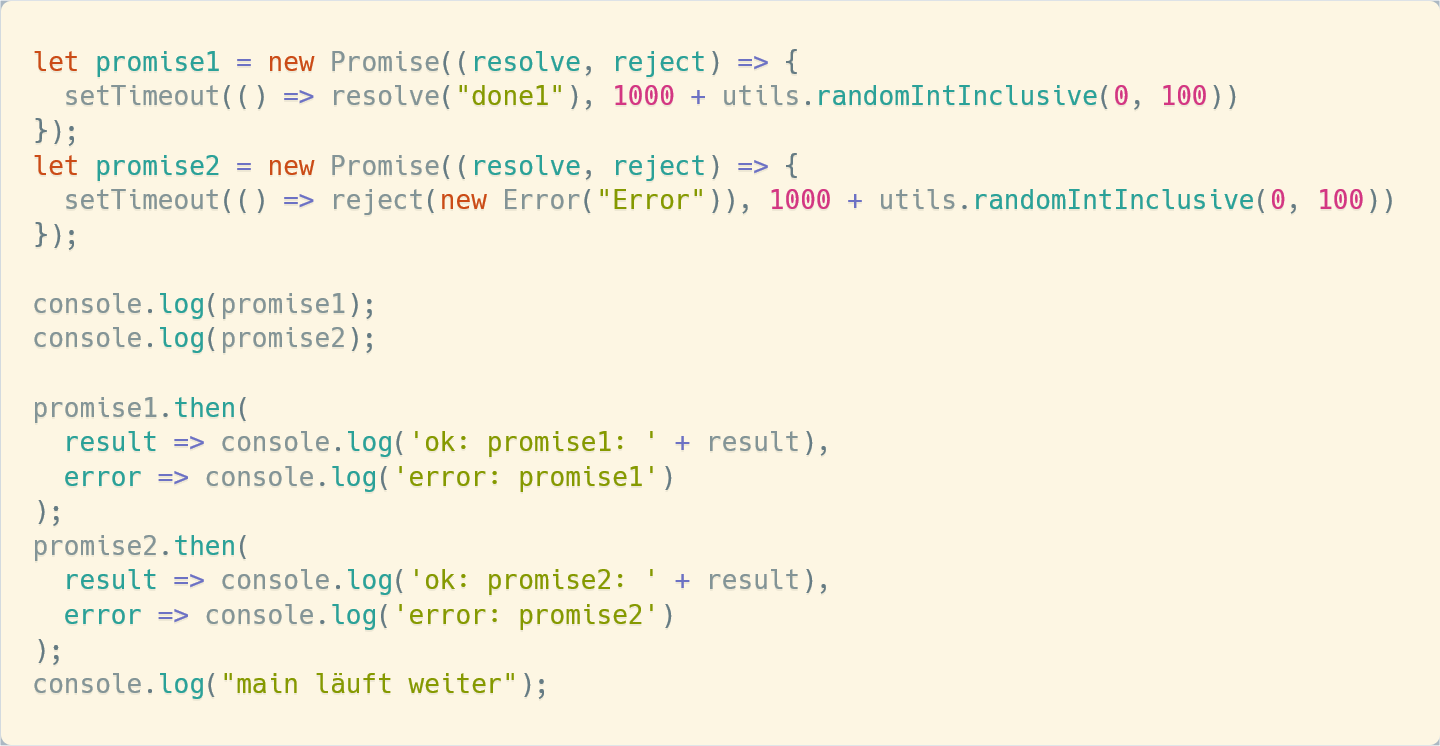
\includegraphics[scale=.22]{fig/promises2a.png}\\[-2.9cm]
    \begin{columns}
      \begin{column}{0.5\textwidth}
        \mbox{}
      \end{column}
      \begin{column}{0.3\textwidth}
        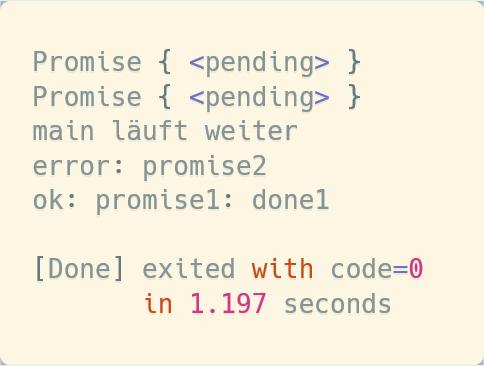
\includegraphics[scale=.21]{fig/promises2b.png}
      \end{column}
    \end{columns}
  \end{center}
\end{frame}

\begin{frame}{Asynchrone Ausführung}
  \begin{itemize}
    \item Entkopplung von Callback-Funktion
  \end{itemize}
  \begin{center}
    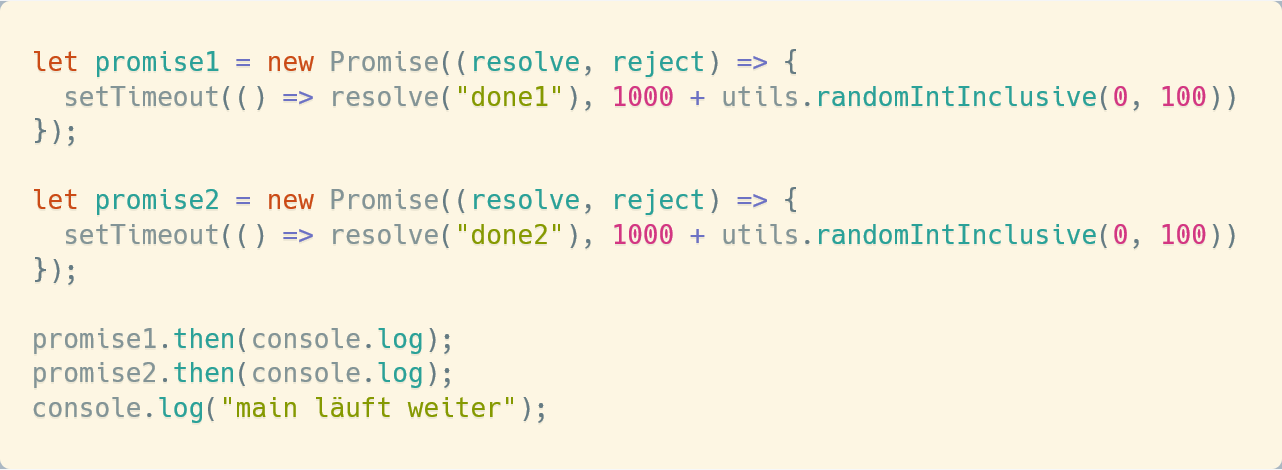
\includegraphics[scale=.24]{fig/promises3.png}\\[.2cm]
    \begin{columns}
      \begin{column}{0.48\textwidth}
        Erster Durchlauf\\[.2cm]
        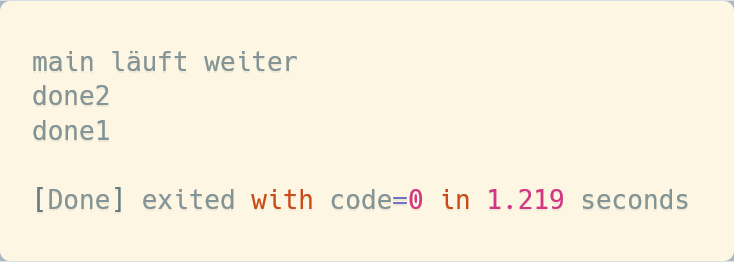
\includegraphics[scale=.21]{fig/promises4.png}
      \end{column}
      \begin{column}{0.48\textwidth}
        Erneuter Durchlauf\\[.2cm]
        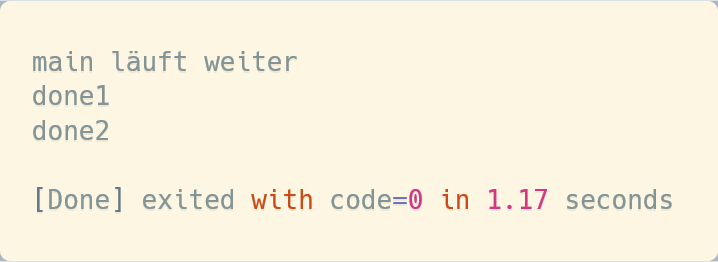
\includegraphics[scale=.21]{fig/promises5.png}
      \end{column}
    \end{columns}
  \end{center}
\end{frame}

\begin{frame}{Synchronisierung 1 -- async/await}
  \vspace*{-.3cm}
  \begin{itemize}
    \item await geht nur in async-Funktionen
  \end{itemize}
  \begin{center}
    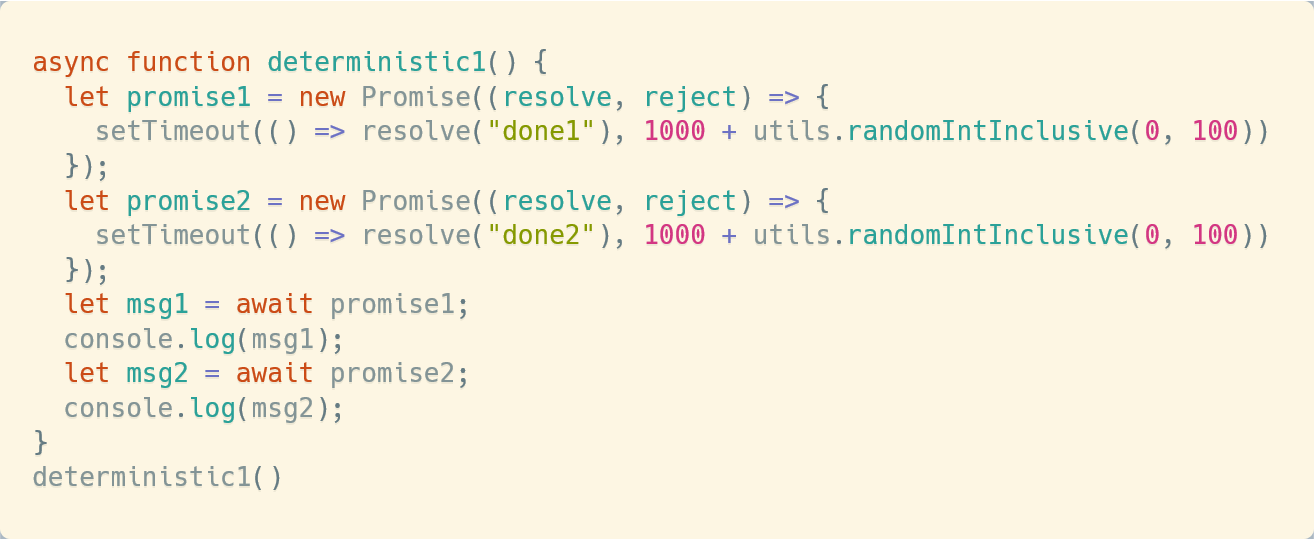
\includegraphics[scale=.24]{fig/promises6.png}\\[-.2cm]
    \begin{columns}
      \begin{column}{0.48\textwidth}\\
        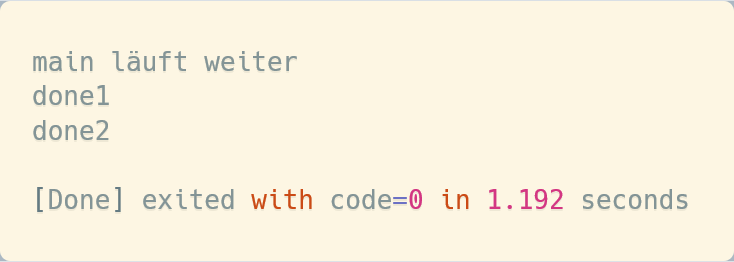
\includegraphics[scale=.21]{fig/promises7.png}
      \end{column}
      \begin{column}{0.48\textwidth}
        \begin{itemize}
          \item Promise 1 und 2 laufen asynchron
          \item Ausgabe der Ergebnisse synchronisiert
        \end{itemize}
      \end{column}
    \end{columns}
  \end{center}
\end{frame}

\begin{frame}{Synchronisierung 2 -- async/await}
  \begin{center}
    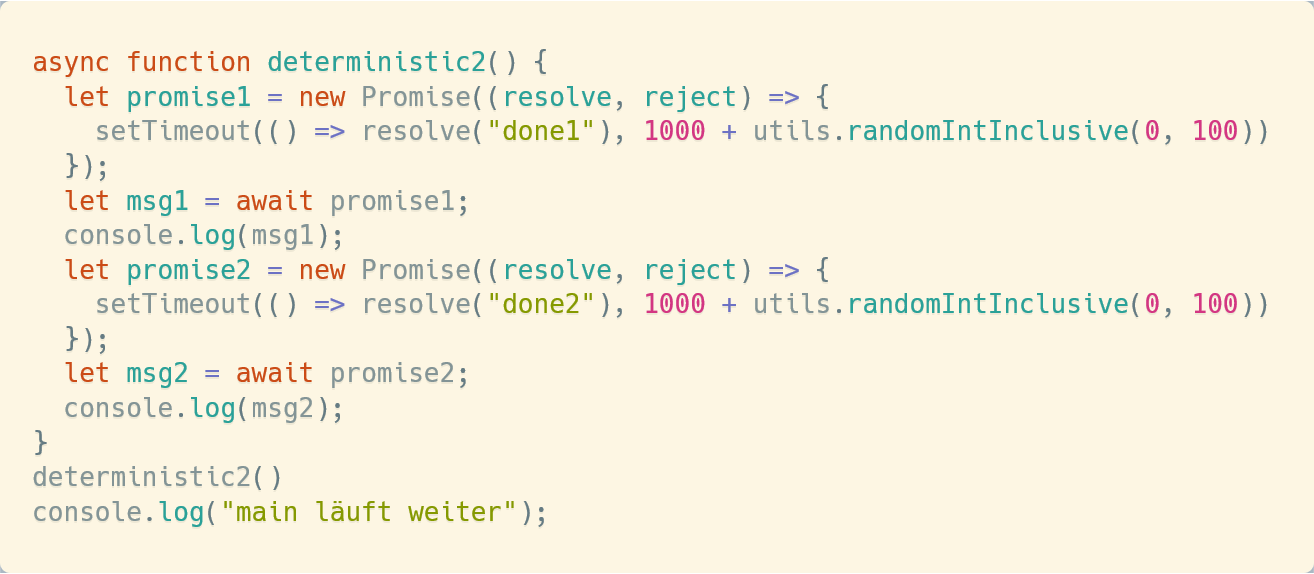
\includegraphics[scale=.24]{fig/promises8.png}\\[-.2cm]
    \begin{columns}
      \begin{column}{0.48\textwidth}\\
        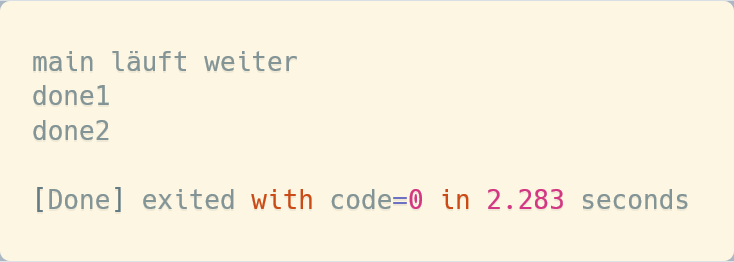
\includegraphics[scale=.21]{fig/promises9.png}
      \end{column}
      \begin{column}{0.48\textwidth}
        \begin{itemize}
          \item Erst läuft Promise 1 dann Promise 2
          \item Doppelte Ausführungszeit!
        \end{itemize}
      \end{column}
    \end{columns}
  \end{center}
\end{frame}

\begin{frame}{Promisification}
  \begin{columns}
    \begin{column}{0.30\textwidth}\\
      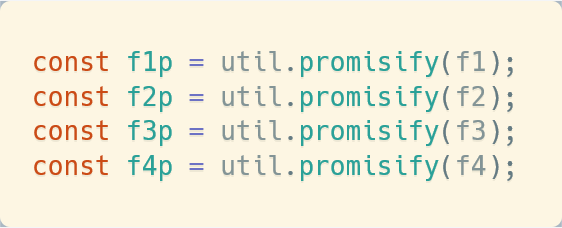
\includegraphics[scale=.21]{fig/promify1.png}
    \end{column}
    \begin{column}{0.5\textwidth}\\
      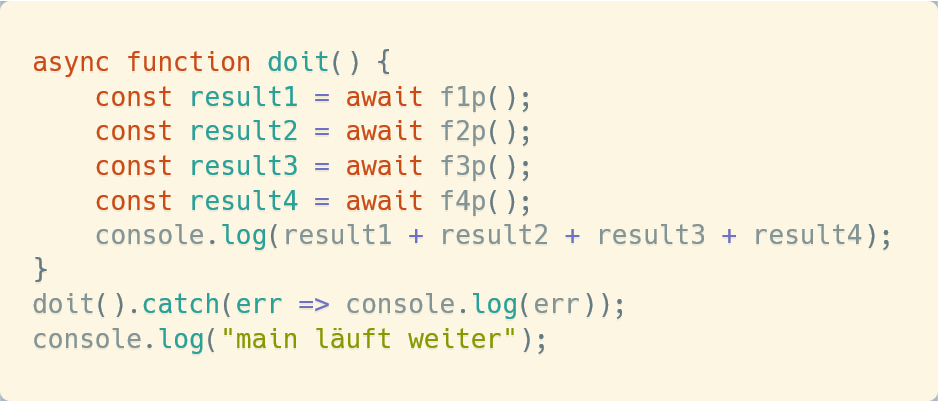
\includegraphics[scale=.21]{fig/promify2.png}
    \end{column}
  \end{columns}
  \begin{center}
    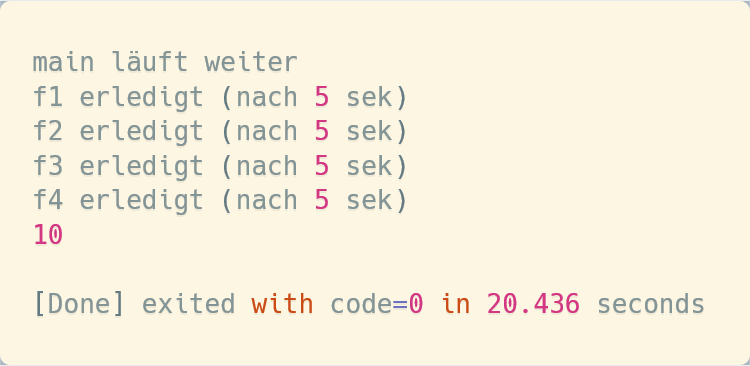
\includegraphics[scale=.24]{fig/promify3.png}
  \end{center}
\end{frame}


\section{JavaScript und Hana}

\begin{frame}{Datenbanktabelle}
  \begin{center}
    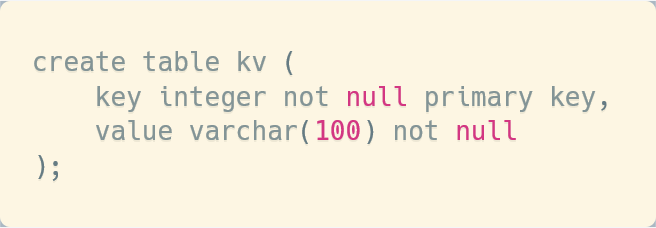
\includegraphics[scale=.3]{fig/key-value-tabelle.png}\\[.3cm]
    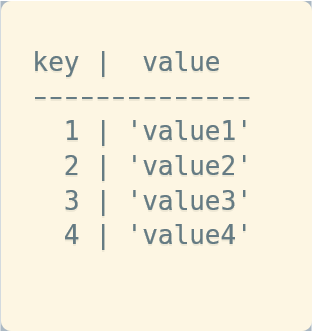
\includegraphics[scale=.3]{fig/key-value-daten.png}
  \end{center}
\end{frame}

\begin{frame}{Callback-Variante}
    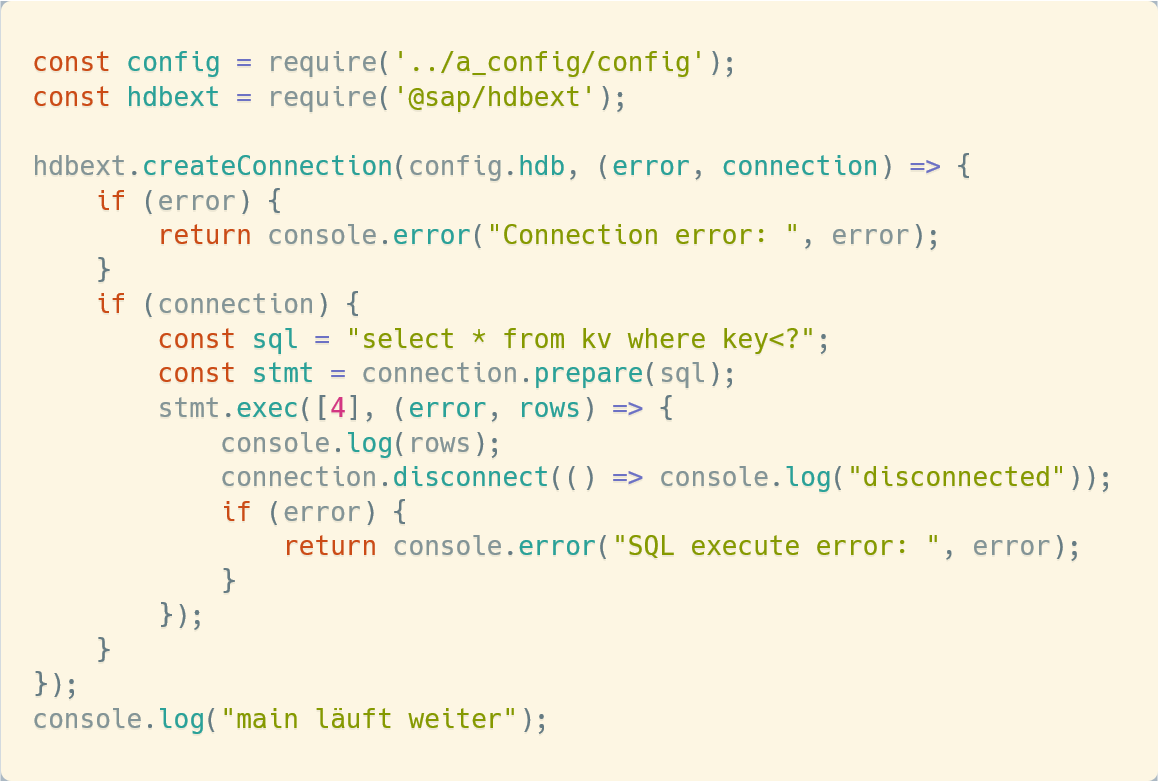
\includegraphics[scale=.24]{fig/hdb-cb.png}\\[-1.6cm]
    \hfill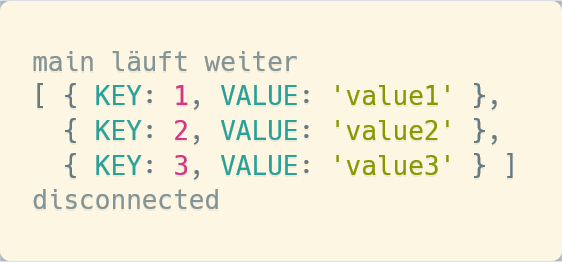
\includegraphics[scale=.21]{fig/hdb-cb-result.png}
\end{frame}

\begin{frame}{Promisified Variante}
  \begin{center}
    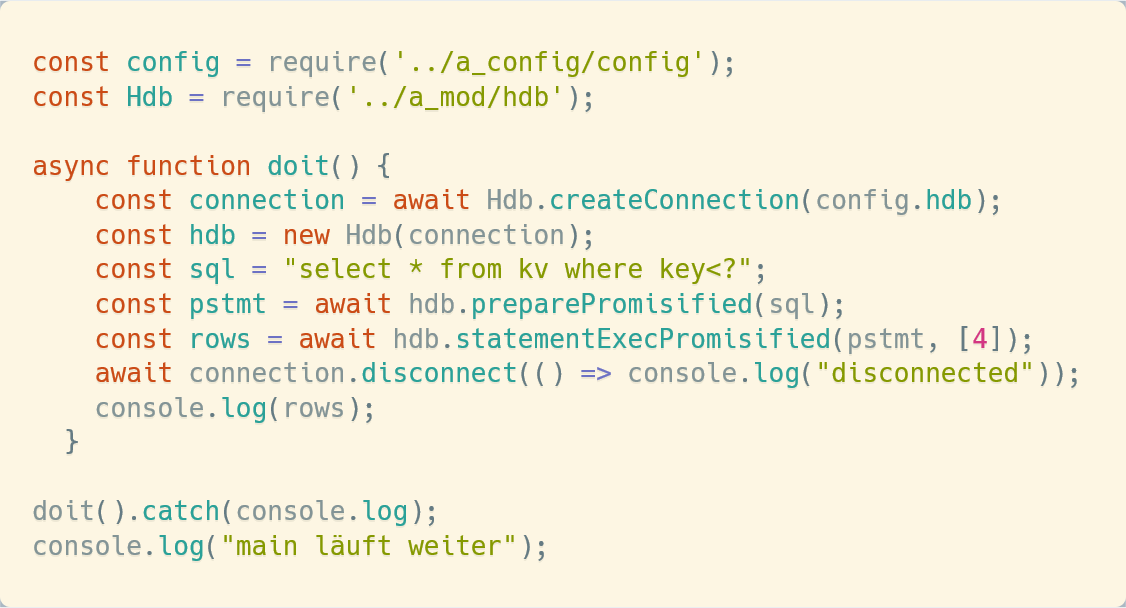
\includegraphics[scale=.24]{fig/hdb-promise.png}
  \end{center}
\end{frame}

\begin{frame}{Hdb Klasse (1)}
  \begin{center}
    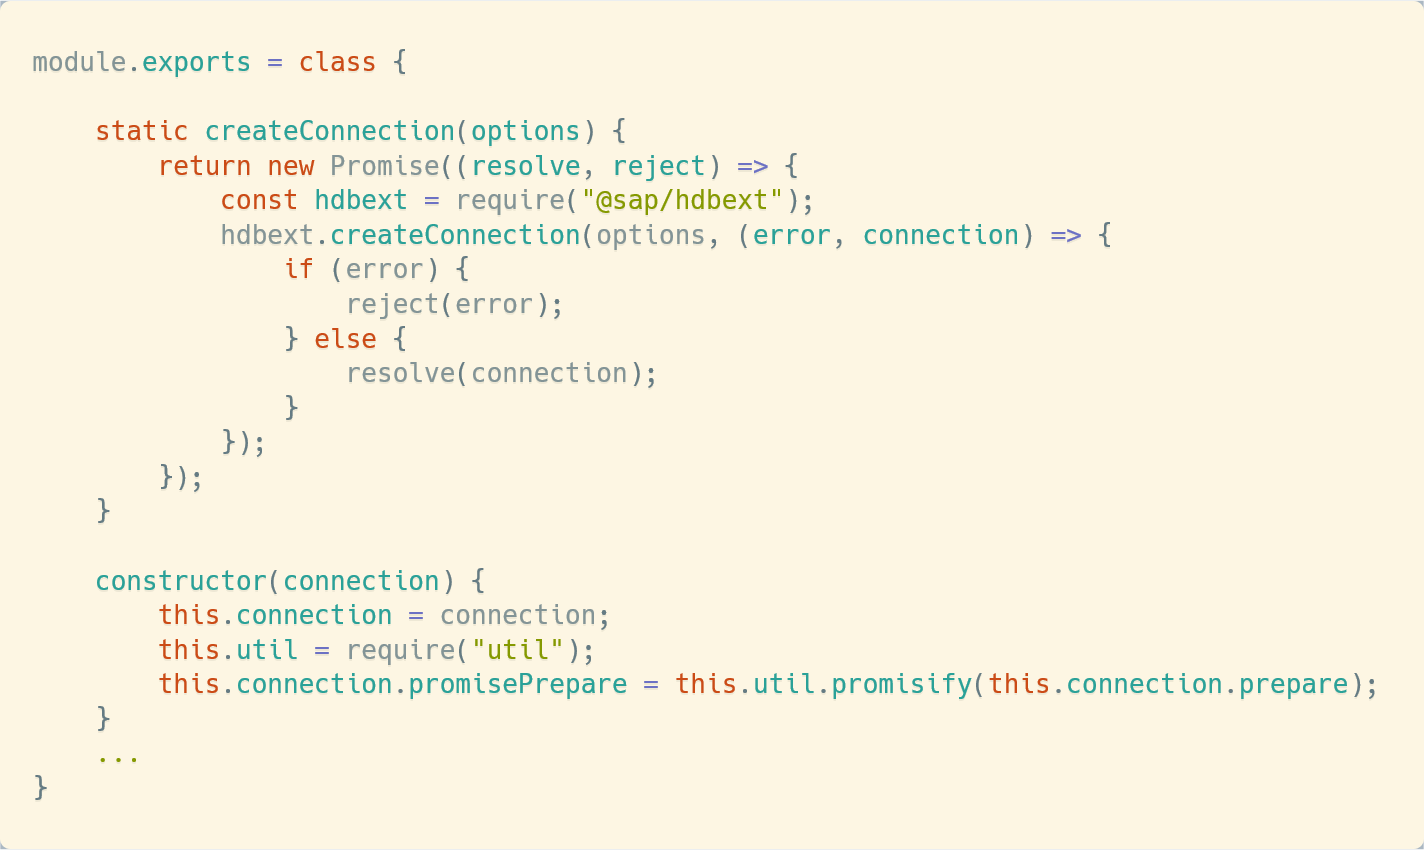
\includegraphics[scale=.22]{fig/hdb-class1.png}
  \end{center}
\end{frame}

\begin{frame}{Hdb Klasse (2)}
  \begin{center}
    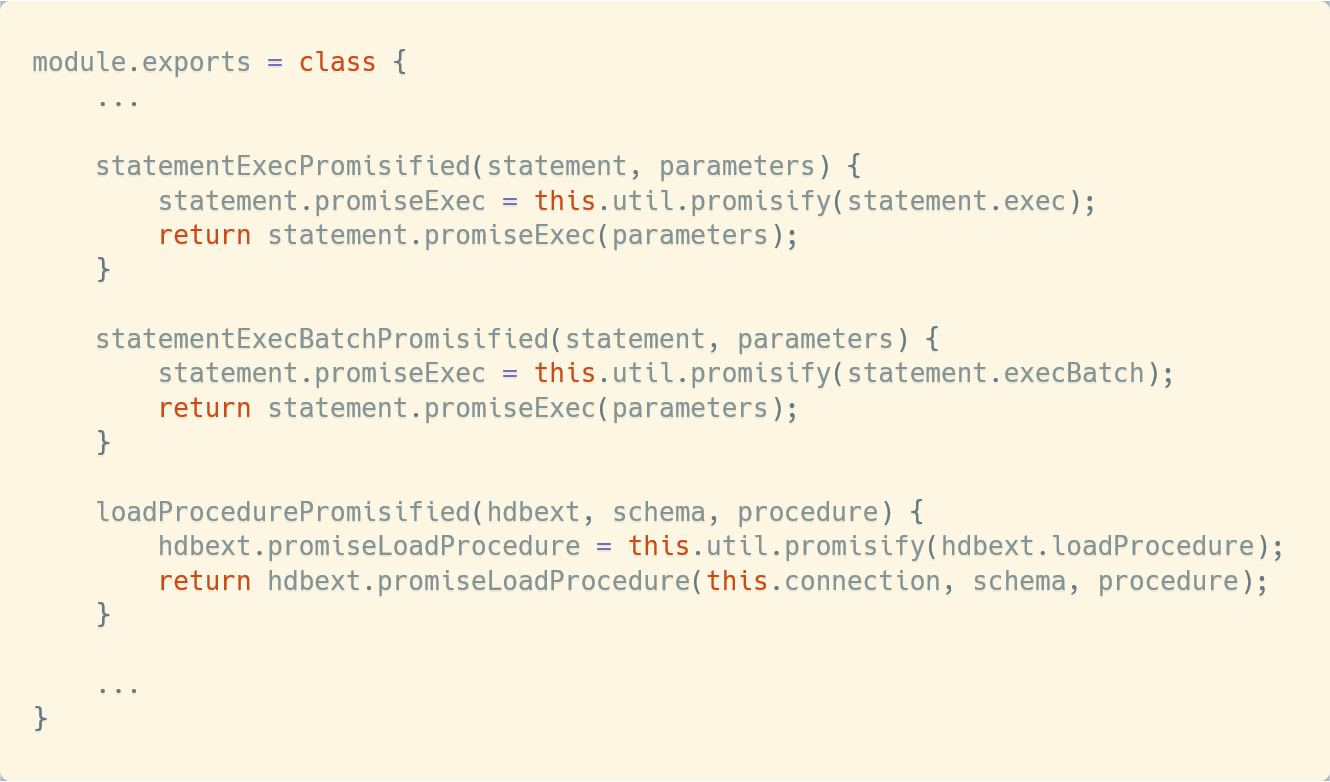
\includegraphics[scale=.22]{fig/hdb-class2.png}
  \end{center}
\end{frame}

\begin{frame}{DB Op}
  \begin{center}
    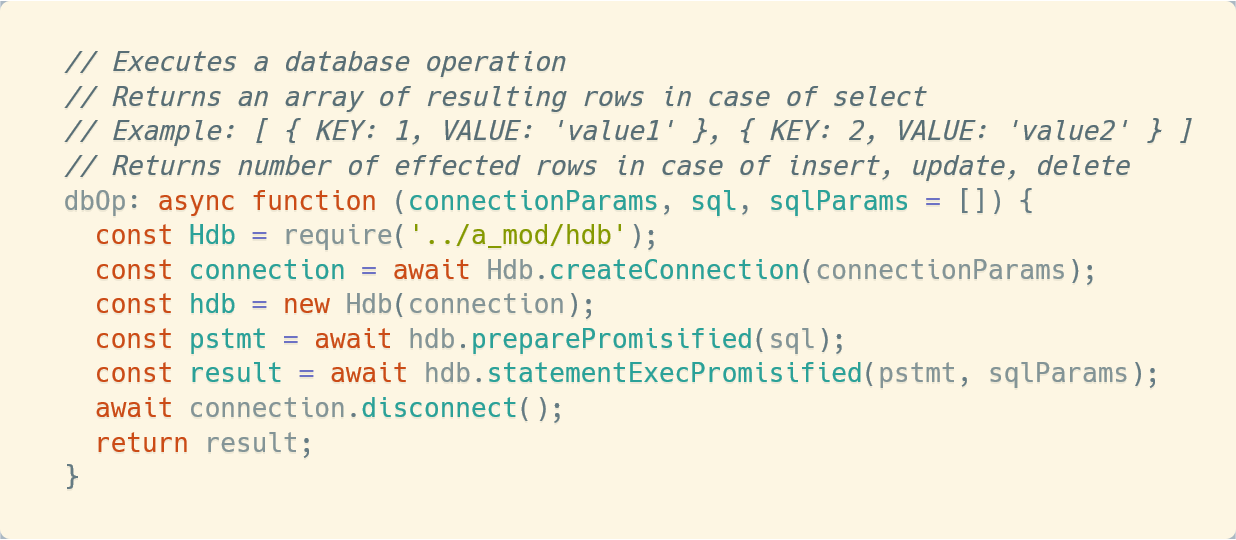
\includegraphics[scale=.24]{fig/db-op.png}
  \end{center}
\end{frame}

\begin{frame}{DB Op Select}
  \begin{center}
    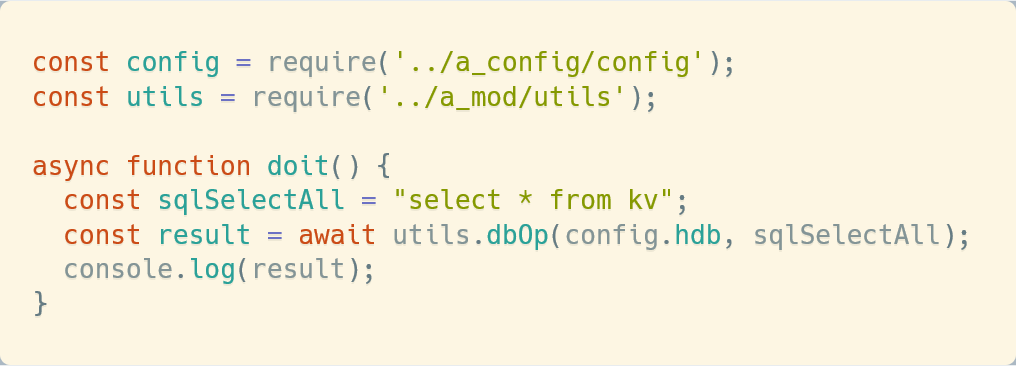
\includegraphics[scale=.24]{fig/db-op-select.png}
  \end{center}
\end{frame}

\begin{frame}{Textanalytics}
  \begin{center}
    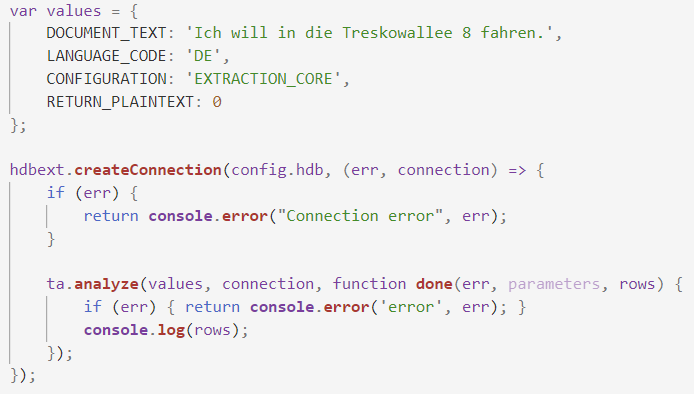
\includegraphics[scale=.45]{fig/ta1.png}\hspace*{.2cm}
    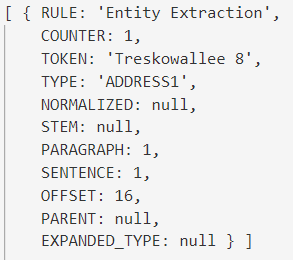
\includegraphics[scale=.45]{fig/ta2.png}
  \end{center}
\end{frame}


\section{Web Services / HTTP Server}

\begin{frame}{Web Framework Express}
  \begin{center}
    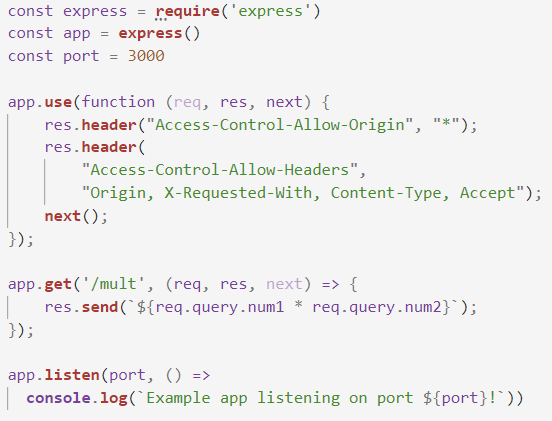
\includegraphics[scale=.5]{fig/express.png}
  \end{center}
\end{frame}

\begin{frame}{VS Code -- Rest Client}
  \begin{center}
    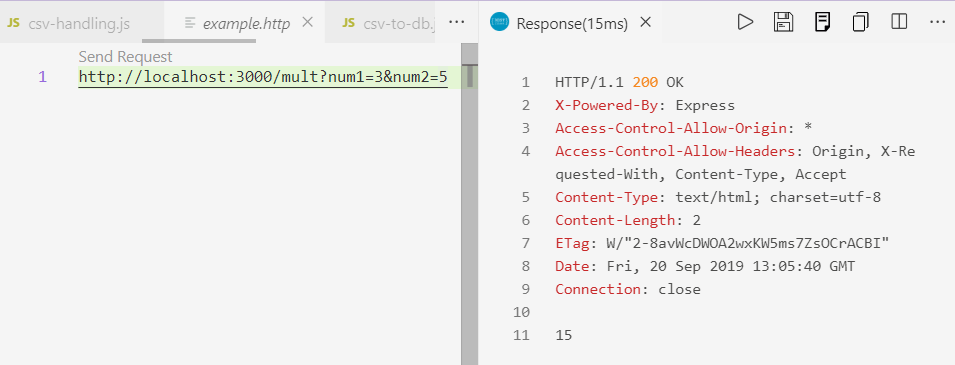
\includegraphics[scale=.45]{fig/express-call.png}
  \end{center}
\end{frame}


\section{Quellen}
\begin{frame}{Quellen}
  \begin{itemize}
    \item The Modern JavaScript Tutorial\\ \url{http://javascript.info/}
    \item SAP HANA Platform - Help Portal\\ \url{https://help.sap.com/viewer/product/SAP_HANA_PLATFORM/2.0.04/en-US}
    \item The Node.JS Sytem \\ \url{https://mobile.twitter.com/TotesChaoticMeh/status/494959181871316992}
  \end{itemize}
\end{frame}


\end{document}

\begin{frame}{xxx}
  \begin{itemize}
    \item
  \end{itemize}
  \begin{center}
    \includegraphics[scale=.5]{fig/xxx.png}
  \end{center}
\end{frame}

